\title{\textbf{Haiku}\\Operating System Report}
\author{COMP 3000\\ \\Troy Hildebrandt\\Nima Hoda}
\date{\today}

\documentclass{article}

\usepackage{cite}
\usepackage{url}
\usepackage{graphicx}
\usepackage{subfig}
\usepackage{booktabs}

\newcommand{\toprul}{\toprule[1.2pt]}
\newcommand{\tmidrul}{\midrule[1.2pt]}
\newcommand{\bottomrul}{\bottomrule[1.2pt]}
\newcommand{\figref}[1]{Figure~\ref{fig:#1}}

% Page setup
% Shamelessly stolen from Pat Morin's Open Data Structures
\setlength{\textheight}{8.5in}
\setlength{\textwidth}{6in}
\setlength{\topmargin}{-0.375in}
\setlength{\oddsidemargin}{.25in}
\setlength{\evensidemargin}{.25in}
\setlength{\headheight}{0.200in}
\setlength{\headsep}{0.4in}
\setlength{\footskip}{0.500in}
\setlength{\parskip}{1.5ex}
\setlength{\parindent}{1.25cm}
%\flushbottom

\begin{document}
\maketitle

\section{Background}

Haiku is a portable \cite{HaikuFaq} free and open source
\cite{HaikuDevFaq} OS (Operating System) for the 32-bit x86 architecture
\cite{HaikuFaq} targeting personal computing \cite{HaikuAbout}.  It
was originally named OpenBeOS after BeOS \cite{HaikuWiki}, the
short-lived proprietary OS developed by Be, Inc. throughout the 1990s,
which focused on digital media work
\cite{BeosWiki}.

BeOS boasted an object-oriented C++ API (Application Programming
Interface), a fully integrated graphical user environment, a modern
multi-processing, pre-emptively multi-tasking kernel, a journaling
file system with a relational database-like metadata
facility \cite{BFSWiki} and included partial POSIX compatibility.
However, despite having a devoted niche user base, it could not yield
a profit for Be, Inc. and, in 2001, was acquired by Palm, Inc., ending
further BeOS development \cite{BeosWiki}.

Disappointed with the loss, a group of BeOS enthusiasts began an
effort to rewrite BeOS as a free and open source project
\cite{BeosWiki, HaikuHistoryWiki}.  In 2004 the open source effort was
renamed Haiku, after the three line Japanese form of poetry which
appeared on occasion in BeOS error messages \cite{HaikuFaq,
HaikuHistoryWiki}.

Haiku takes its inspiration from BeOS \cite{HaikuAbout} and aims to
recreate both the BeOS technologies and end user experience
\cite{HaikuFaq}.  Haiku uses the same window decoration style and
color as BeOS \cite{HaikuWiki, BeosWiki} and aims to create a
unified, cohesive user interface \cite{HaikuAbout, HaikuHIG,
HaikuIcon} reflecting the ``core qualities'' of ``elegance'' and
``simplicity'' found in BeOS \cite{HaikuFaq}.  Haiku also directly
incorporates two core BeOS user interface elements, the Tracker, a
file manager, and the Deskbar, a taskbar, which were open sourced by
Be, Inc. in 2001 \cite{HaikuFaq}.  Haiku also reimplements the
object-oriented C++ BeOS API\cite{HaikuWiki} as well as the Be File
System with, its advanced meta-data capabilities \cite{BFSWiki}.

Haiku is targeted towards the personal computer user
\cite{HaikuAbout}.  As such, it includes a fully integrated GUI
(Graphical User Interface) environment, rejecting the stacked nature
of the X Window System on UNIX-like OSes \cite{HaikuFaq}.  The
personal computing focus is also reflected in Haiku's current lack of
support for multi-user operation, though are plans for such support in
future releases \cite{HaikuFuture}.  Haiku also aims to present a
unified human interface, both in terms of the OS base as well as in
applications developed for Haiku.  This is reflected in the
development and maintenance of comprehensive Haiku human interface and
icon guidelines \cite{HaikuHIG, HaikuIcon}.

Haiku currently only supports the 32-bit x86 architecture, though
ports to other platforms, including x86-64, are being developed and
may be supported in the future \cite{HaikuFaq}.  On 32-bit x86, Haiku
aims for full source and binary compatibility with 32-bit x86 BeOS
applications.  Several major BeOS R5 applications already run
successfully on Haiku, including Opera, Firefox and Quake II
\cite{HaikuWiki}.  POSIX compatibility is also a Haiku goal
\cite{HaikuFuture, HaikuIncContracts}, as are the development of a
BSD (Berkeley Software Distribution)-style ports
collection \cite{HaikuPorts}, which would simplify the building of 3rd
party open-source software and a full package management system to
manage installation and dependency resolution of 3rd party
software \cite{HaikuR1A3Notes}.

Haiku development is centered around the Haiku Project, an
international community of volunteers \cite{HaikuAbout}.  The project
maintains mailing lists, forums, IRC (Internet Relay Chat)
channels, \cite{HaikuComm} source code repositories \cite{HaikuGetSvn}
and several websites, including the following:
\begin{itemize}
  \item \url{http://www.haiku-os.org/} -- the main project website
  \item \url{http://api.haiku-os.org/} -- containing Haiku API documentation
  \item \url{http://dev.haiku-os.org/} -- the Haiku project management
    system
  \item \url{http://www.haiku-files.org/} -- an archive of nightly
    builds for Haiku
  \item \url{http://ports.haiku-files.org/} -- the Haiku ports collection
    project management system
\end{itemize}

There are 81 developers with commit access to the Haiku source code
repository, with the top contributors ranking in the thousands of
commits over many years \cite{HaikuContrib}.  The source code is
revision controlled by a subversion repository and managed by Trac
\cite{HaikuDevStart}.  Write access to the repository is granted to
contributors on the basis of past contributions \cite{HaikuDevStart}.

In addition to voluntary contributions, the Haiku Project has also
participated in GSOC (Google Summer of Code)---a program that provides
stipends to students who contribute to open-source software
\cite{GSOCWiki}---every year since 2007 \cite{HaikuGSOC}.  In 2010,
Haiku took contributions from seven students through GSOC
\cite{HaikuGSOC2010}.  Contributors are also sometimes contracted to
work full-time on Haiku, allowing them to dedicate large continuous
blocks of time to Haiku development \cite{HaikuIncContracts}.
Contract lengths have mostly been limited to several weeks but also
include a recently awarded six month contract
\cite{HaikuLongContract}.

The Haiku Project is supported financially by Haiku, Inc., a 501(c)(3)
charitable non-profit corporation founded in 2003 by Michael Phipps in
New York State's Division of Corporations \cite{HaikuIncAbout,
HaikuInc}.  Haiku, Inc., funded through donations, has a 2011
operating budget of \$25,500 \cite{HaikuIncDocs}.  Donations to Haiku,
Inc. come almost entirely from private individuals, either directly to
Haiku, Inc. or through ``bounties'' and ``Thank You Awards'' from
HaikuWare \cite{HaikuIncDonors, HaikuWareBounties}, a repository of
pre-built software for Haiku as well as a hub for Haiku end-users
\cite{HaikuWareAbout}.

Haiku Release 1 Alpha 3 was published on June 20, 2011
\cite{HaikuRelease}.  It is available for free download from various
FTP (File Transfer Protocol) and HTTP (Hypertext Transfer Protocol)
mirrors in the following formats \cite{HaikuGet}:
\begin{itemize}
\item ``Anyboot'' images -- which may be written to and booted from
  USB (Universal Serial Bus) flash drives, hard disk drives or CD
  (Compact Disc)/DVD media
\item ISO (International Organization for Standardization) images
  -- which may be written to CD media
\item VMDK (Virtual Machine Disk Format) images -- which are virtual
  machine disk files compatible with VMWare products as well as QEMU
  and VirtualBox \cite{VMDKWiki}
\end{itemize}
Any of the image formats may be used live, to try Haiku without
installing it, or to install Haiku to another disk volume
\cite{HaikuGet}.  The Haiku alpha release is also available for order
on a ``commemorative'' CD from Haiku, Inc. for a minimum donation of
\$10 per disc \cite{HaikuIncOrder}.  Source code for this release is
also available for download in compressed archived form
\cite{HaikuR1A3Src}.

The latest Haiku source code can be obtained directly from the source
code repository \cite{HaikuGetSvn} and nightly snapshot builds are
available as downloadable images from the Haiku Files archive
\cite{HaikuFiles}.

The Haiku release (Anyboot) is approximately 250MB (megabytes) in size
compressed \cite{HaikuGet} and 700MB uncompressed.  The installed
system also takes up about 700MB of disk space, not including the size
of a swap file, which is 2GB (gigabytes) by default.  The source
distribution is split into two files.  One containing the Haiku build
tools, comprised almost entirely of customized third party software
(e.g. GCC (GNU Compiler Collection), binutils) and having an
uncompressed size of about 530MB, and the other containing the Haiku
system sources proper and having approximately the same uncompressed
size \cite{HaikuR1A3Src}.  The Haiku system sources contain about 5.5
million lines of C and C++ code and headers, not including blank or
comment lines, as reported by CLOC (Count Lines of Code) \cite{Cloc}.

\section{Installation Procedure}

For the purposes of testing, installation was performed on an Oracle
VirtualBox setup, in this specific case using Windows 7 64bit host as
a host OS.  The OS was set to Other/Unknown, and 512MB of memory was
allotted for Haiku to use. 4GB was the amount of hard-disk space I
chose to allow Haiku to use, and ``Dynamically expanding storage'' was
selected just in case.

\begin{figure}[h]
\centering
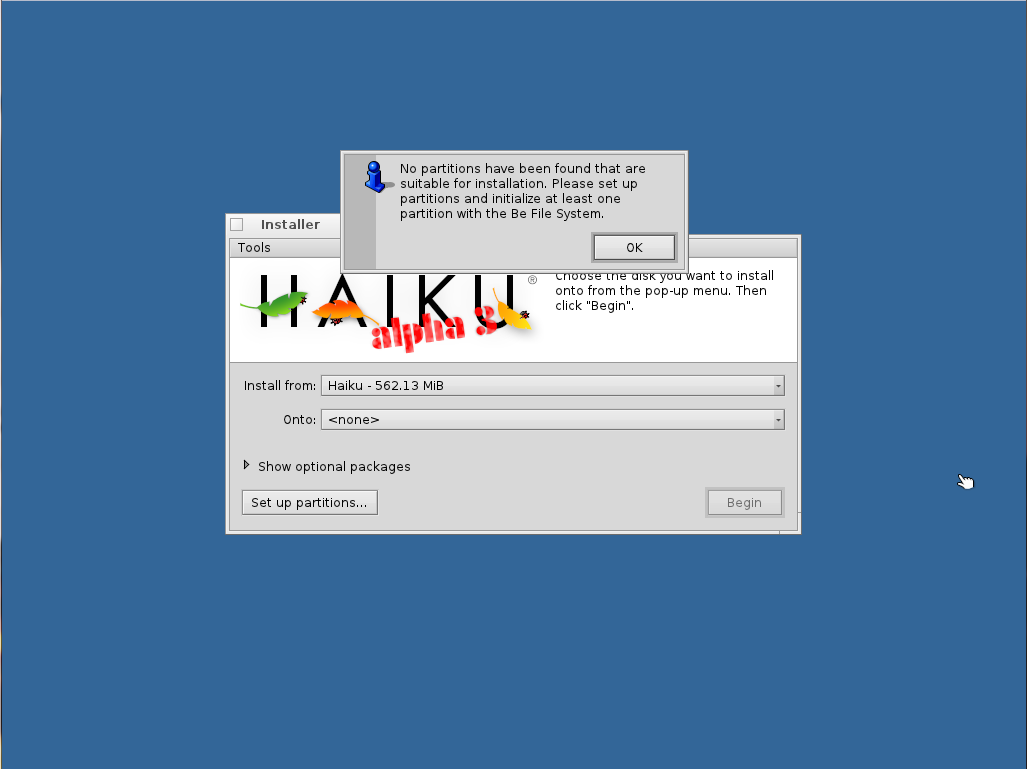
\includegraphics[width=0.9\textwidth]{figs/install-partition.png}
\caption{Partition selection in the Haiku installer.}
\label{fig:install-partition}
\end{figure}

\begin{figure}[h]
\centering
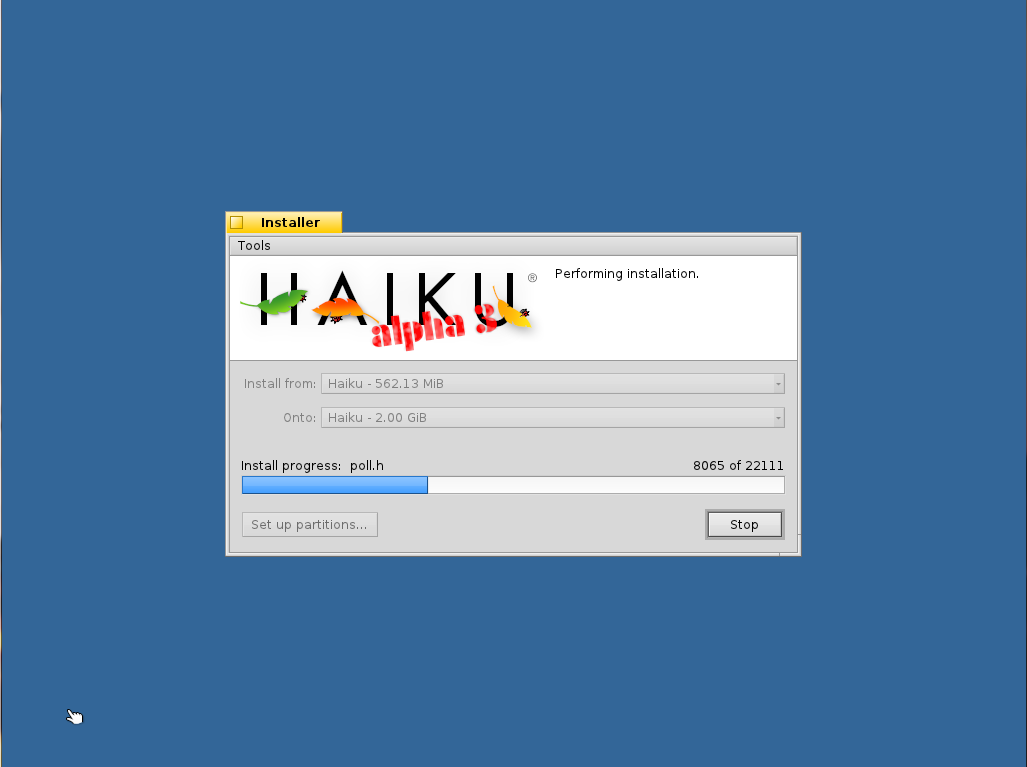
\includegraphics[width=0.5\textwidth]{figs/install-progress.png}
\caption{The Haiku installer copying files and displaying installation
  progress.}
\label{fig:install-progress}
\end{figure}

Installation began by selecting the Haiku disc ISO to be used for the
secondary IDE (Integrated Drive Electronics) device in the Storage
Settings for my Haiku guest, and a first boot was initiated.  After a
simple language select, a quick and painless format of my 4GB
partition to the Be file system (\figref{install-partition}), my
partition was ready to be selected from a drop down list and the
install could begin (\figref{install-progress}).  This process could
simply not have been more painless, and there were absolutely no
surprises or hurdles to overcome during the process.  After the
progress bar reached the end, I chose the ``Quit'' option and the
system rebooted to be used for the first time.

\section{Startup}

\begin{figure}[h]
\centering

\includegraphics[width=0.5\textwidth]{figs/startup.png}
\caption{The Haiku boot screen.}
\label{fig:startup}
\end{figure}

The first start-up presents the user with a screen showing the Haiku
logo, and a series of logos that go from monochrome to full color in
sequence to indicate progress during boot-up (\figref{startup}).
Given this execution combined with the artistic styling of the logos,
this is very reminiscent of Maxis' The Sims series of games.

After a noticeably rapid boot process, users familiar with Haiku's
inspiration and spiritual predecessor, BeOS, will be greeted instantly
with both familiar desktop and icon styling along with the Tracker,
one of very few things that made a direct translation from BeOS to
Haiku as part of being open-sourced in 2001 \cite{HaikuFaq}.

A stark install process gives way to very few options, and with very
little additional effort, Haiku is for all intents and purposes ready
for use.  The time taken from start to finish in setting up an
installation of Haiku under VirtualBox is roughly five minutes.

\section{Basic Operation}

Haiku comes pre-installed with a host of applications that the average
user may use, the most important of which is likely its pre-installed
browser, titled WebPositive.  Haiku is aimed at ``personal
computing,'' and given this vague definition, seems at first glance to
fulfill the needs of an average light user. The web browser will be
the obvious first stop for most users looking to get more software and
make their Haiku experience a more entertaining or productive one.
	
This is where the first very minor problem was encountered, and it was
a network related issue. Haiku refused to recognize the default
network card that VirtualBox had chosen to virtualize, and so a quick
shutdown and modification of this setting to an Intel Pro/1000 MT
desktop card solved the problem immediately.
	
\begin{figure}[h]
\centering
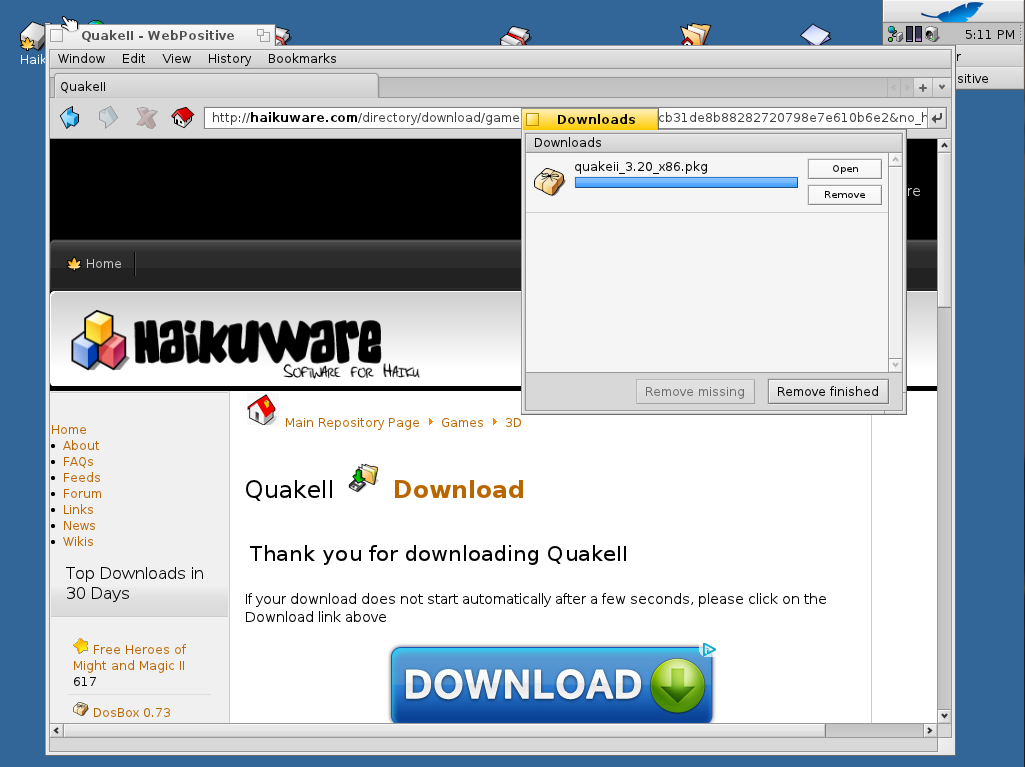
\includegraphics[width=0.9\textwidth]{figs/using-quake-download.png}
\caption{WebPositive, the Haiku web browser, downloading Quake II from
  HaikuWare.}
\label{fig:using-quake-download}
\end{figure}

A user looking to expand their selection of installed software will
likely end up at the site HaikuWare (located at
http://www.haikuware.com).  Considering my resounding disinterest in
word-processing or productivity programs, I decided to hunt down a
Haiku-compatible version of a classic favorite of mine, id Software's
Quake II (\figref{using-quake-download}).  Interestingly enough, the
claim from the download page at Haikuware for Quake II claims it is
the same version that used to be found on BeDepot.
	
\begin{figure}[h]
\centering
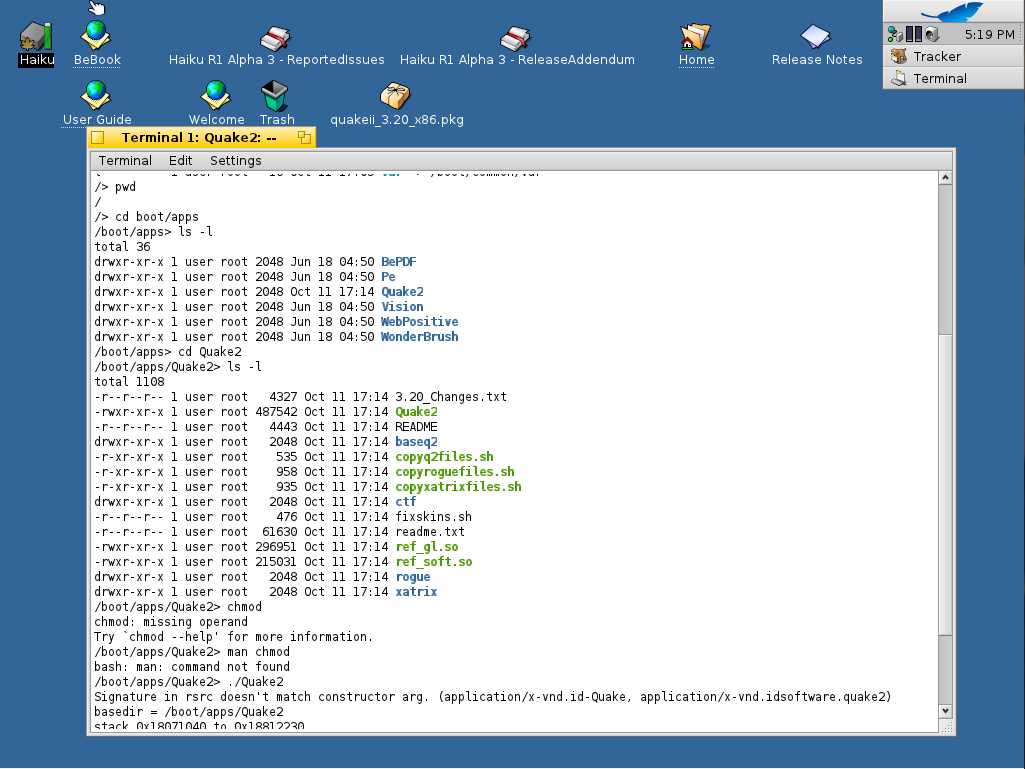
\includegraphics[width=0.9\textwidth]{figs/using-terminal.png}
\caption{A Bash terminal window open in Haiku.}
\label{fig:using-terminal}
\end{figure}

Following the download's completion, the most obvious feature was its
file extension, .PKG. Not recognizing this immediately as a BeOS
installation package, a double click revealed a very simple
auto-install process that I promptly allowed to install to its default
directory, /boot/apps.  The file system hierarchy in BeOS/Haiku is
very similar to that of a Unix OS, despite Haiku not being a Unix
based operating system, and as such the directory structure looks very
similar to Unix systems.  Haiku comes with a Bash terminal, with
instantly recognizable Unix commands such as ls, chmod, pwd, and many
others (\figref{using-terminal}).  The mounting of a CD is automatic,
and very easily accessible once inserted, either from a link on the
desktop, or from the root directory, based on what the name of the CD
is.  In this case, I could access the files on the Quake II CD from
/Quake2, and the files from the installation of BeOS Quake II at
/boot/apps/Quake2.

\begin{figure}[h]
\centering
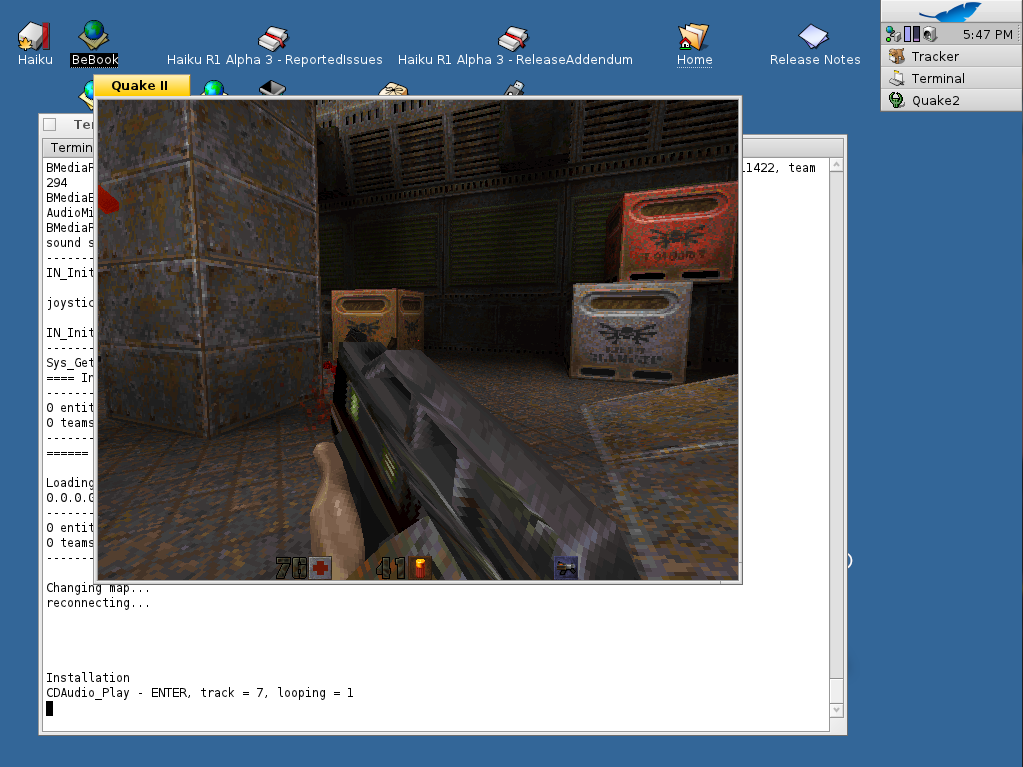
\includegraphics[width=0.5\textwidth]{figs/using-quake-play.png}
\caption{Quake II for BeOS running on Haiku.}
\label{fig:using-quake-play}
\end{figure}
	
After copying the contents of a full Windows installation of Quake II
into Haiku via USB drive (which again was instantly recognized and
mounted), I started it up. Copying from a previously installed Windows
version was necessary because the CD was the Windows version, and
availability of a native BeOS installer is unlikely.

The first noticeable problems were both the obviously broken and
ear-piercing sound which caused me to mute my PC (Personal Computer),
and the excruciatingly slow Mesa software OpenGL implementation that
the game defaulted to.  This is a result of no Guest Additions and no
virtualized OpenGL 3D-acceleration, and as a result, I switched to
pure software rendering mode which ended up working out nicely
(\figref{using-quake-play}).  However, attempting to start a game
causes a crash, and while playing the beginning demo the game will
occasionally crash as well.  I'm not sure if this is a result of it
being a BeOS executable, the fact that I'm running it in VirtualBox,
or just that the BeOS/Haiku executable of Quake II isn't quite ready
for prime time yet.  I was nevertheless still impressed to see it
running in any capacity in Haiku.
	
Most people will at some point want to watch a video on Youtube, or at
least some Flash-based video website.  If Haiku was going to be of any
use to the average personal computer user, I was going to need to
determine whether or not Youtube was a viable option in Haiku.  I set
about trying to download a new browser from Haikuware to spruce up my
browsing experience, and to find out how simple the installation of
new software would be. The unfortunate discovery was that there is a
high degree of difficulty finding and installing new software in
Haiku, partly due to the tiny number of apps available to it that both
run natively, and are easy to install.

There is a small selection of browsers available for Haiku directly
from Haikuware, but they're mostly old versions of browsers
(i.e. Firefox 2.0 since Firefox 3 still isn't fully ported, as well as
older versions of Opera) that still don't have proper plugin support
for things like Flash.  Since Flash is closed-source, open-source
versions of it like Gnash are made, but are still largely unsupported
and not optimal.  This makes something like watching Youtube a more
massive undertaking than most basic users will be capable of, since
getting Flash support in a web browser in Haiku is a task in itself.
This speaks poorly to Haiku's goal to be for ``personal computing,''
considering how many more popular operating systems provide this basic
functionality.

\section{Usage Evaluation}

While a seemingly faithful recreation of the original BeOS and an
impressive piece of work in its own right, Haiku falls short of its
goals to be for ``personal computing'' by simply not having enough
software support and lacking in the excellent package distribution
models that many other more popular operating systems provide.  An
interesting OS, and considering it's open source model could
technically be made to do anything if you felt so inclined, but the
types of users who would delve into source code to coax Haiku into
being more useful aren't the sort of people I feel the Haiku
developers are speaking to when they describe it vaguely as being for
``personal computing.''

\section{Software Packaging}

Despite starting life as OpenBeOS over ten years ago, Haiku is still
lacking a comprehensive package management system. While a package
management system is currently in the works\cite{HaikuFuturePkgMan},
there is still much to be done before it's ready for widespread
deployment and use\cite{HaikuPkgTodo}. Instead, Haiku has relied on
several alternate techniques and stop-gap technologies to distribute
software packages.

One such stop-gap technology is the \texttt{installoptionalpackage}
script included with Haiku, admitted by the developers of Haiku
themselves as a ``band-aid for the lack of a proper package
manager.''\cite{InstallOptionalPackage} This script provides limited
functionality similar to more complete package management systems,
such as the ability to list not only installed packages, but available
packages as well. The benefit to this script versus other methods of
obtaining software in Haiku is that the software packages available
through \texttt{installoptionalpackage} are sanctioned by the
developers of Haiku, with guaranteed compatibility. A list of packages
can be obtained by simply typing \texttt{installoptionalpackage -l},
and then installation can be done by way
of \texttt{installoptionalpackage -a <packagename>}.

The Haiku development team has attempted to maintain BeOS
compatibility, which includes support for BeOS .PKG files as early as
2007.\cite{OpeningPkgFiles} At this point in time, it looks like
the \textit{PackageInstaller} that comes as part of Haiku for
compatibility with BeOS package files is fully functional, having
personally installed Quake II for BeOS within Haiku through a .PKG
file. This is great, aside from the fact that
the \textit{PackageInstaller} does simply that, installs. Unlike
complete package management systems, which store information on what
packages are installed and allow for simple uninstallation as well,
BeOS .PKG support in Haiku only allows for quick installation.

During BeOS's life span, an application known
as \textit{SoftwareValet} was used for the distribution of BeOS PKG
files. \textit{SoftwareValet} provided software through a centralized
server known as BeDepot\cite{SoftwareValet} and provided functionality
for not only registration, but also software updates of installed
packages. Unfortunately, the PKG format used by SoftwareValet, and
built using the \textit{PackageBuilder} tool, were proprietary and had
to be reverse engineered.\cite{OpeningPkgFiles} This is likely a
contributing factor in the development of an entirely new software
packaging system for Haiku, and an explanation for the rudimentary
support for BeOS software packages.

Another source of software for Haiku is what's known as ports. Ports
of software already available on other systems can be acquired
at \textit{http://ports.haiku-files.org/}. A simple script is
available from this website that allows the quick installation of an
application known as \textit{HaikuPorter}. This program, once
installed, essentially works in much the same way
as \texttt{installoptionalpackage} does, by providing a list of
available ports, and providing automated download of these ports
packages. .BEP (Be Ports) files are used to determine the rules of
downloading, building, and installing Ports packages.\cite{BepFiles}

The process of obtaining software through \textit{HaikuPorter} is a
simple one. Simply obtain the ports tree using \texttt{haikuporter -g}
much like you obtain a list of available packages with something like
Ubuntu's aptitude, or even the very
simple \texttt{installoptionalpackage} script available in Haiku, list
available ports through \texttt{haikuporter -l} and then choose a
piece of software from this tree to install with \texttt{haikuporter
-i <portname>}. The .BEP file provides information for automating the
download, build, and installation procedures.\cite{BepFiles} A major
downside to downloading software available in the ports tree is that
much of the software is incomplete and incompatible with Haiku at this
point in time. \textit{HaikuPorter}, much
like \texttt{installoptionalpackage}, is also still not a substitute
for a proper package management system. It lacks proper update,
registration, and uninstallation functionality commonly associated
with more comprehensive package management
systems. \textit{HaikuPorter} also lacks the ability to automatically
resolve dependencies, simply because its goal isn't to become as
"powerful as Gentoo Portage or the FreeBSD ports system", making this
a low priority.\cite{HaikuPorter}

Unfortunately in many cases, the only way to remove software on Haiku
is to manually remove the directories and files associated with the
application in question. The only alternative to this at this point is
if an uninstallation script was provided to automate the
process.\cite{AppInstallUninstall}

The goal for Haiku as far as software availability and installation is
ultimately to have a proper package management system akin to that
available with popular Linux distributions.\cite{HaikuFuturePkgMan}
According to one of the developers responsible for developing a
solution to package management for Haiku, \textit{HaikuPorter} will
still play a very large role in the future. Haiku package files
(.HPKG) will essentially work to resolve dependencies before
invoking \textit{HaikuPorter} to complete the build and installation
process.\cite{TappeOnPackages}

\section{Major Package Versions}

In this section we will discuss major third party packages included in
Haiku Release 1 Alpha 3.  Third party software is included in the
Haiku base via two main mechanisms: as forks from the upstream version
and as ports using the Haiku ports framework \cite{HaikuR1A3Src}.  The
forks themselves fall into two categories, those tracking an upstream
version, and those maintained by Haiku developers more or less
independently.  In some cases the package is maintained independently
but bits and pieces of newer versions of the package have been merged
in on a piecemeal basis.

The following table summarizes information about the packages we'll be
discussing in this section.

\begin{tabular}{l l l l}
\toprul
\textit{Package} & \textit{Fork} & \textit{Version} & \textit{Latest Stable Release} \\
\tmidrul
NewOS Kernel & Yes & \string~2002 (snapshot)\footnotemark[1] & 20050620\footnotemark[16] \\
\midrule
GNU libc & Yes & \string~2.2.5-2.3.5 (2005)\footnotemark[2] & 2.14.1 (2011-10-07) \\
\midrule
GNU bash & Yes & 4.0.35 (2009-10-24)\footnotemark[3] & 4.2.10 (2011-05-03) \\
\midrule
GNU coreutils & Yes & 8.4 (2010-01-13)\footnotemark[4] & 8.14 (2011-10-12) \\
\midrule
GNU tar & No & 1.25 (2010-11-07)\footnotemark[5] & 1.26 (2011-03-13) \\
\midrule
GNU sed & No & 4.2.1 (2009-06-27)\footnotemark[6] & 4.2.1 (2009-06-27) \\
\midrule
GNU grep & Yes & 2.5.1 (2002-03-26)\footnotemark[7] & 2.9 (2011-06-21) \\
\midrule
GNU make & No & 3.82 (2010-07-28)\footnotemark[8] & 3.82 (2010-07-28) \\
\midrule
OpenSSH & No & 5.8p2 (2011-05-02)\footnotemark[9]  & 5.9p1 (2011-09-06) \\
\midrule
p7zip & No & 9.13 (2010-05-30)\footnotemark[10] & 9.20.1 (2011-03-16) \\
\midrule
bzip2 & No & 1.0.6 (2010-09-20)\footnotemark[11] & 1.0.6 (2010-09-20) \\
\midrule
WebKit & Yes & r57734 (2010-04-09)\footnotemark[12] & r100096 (2011-11-13)\footnotemark[16] \\
\midrule
gcc2 & Yes & 2.95.3 (2001-03-16)\footnotemark[13] & 4.6.2 (2011-10-26) \\
\midrule
gcc4 & Yes & 4.4.4 (2010-04-29)\footnotemark[14] & 4.6.2 (2011-10-26) \\
\midrule
Perforce Jam & Yes & 2.5 (2003-04)\footnotemark[15] & 2.5 (2003-04) \\
\bottomrul
\end{tabular}

\footnotetext[1]{\url{http://newos.org/snapshots/2002/}}
\footnotetext[2]{\url{http://ftp.gnu.org/gnu/libc/}}
\footnotetext[3]{\url{ftp://ftp.gnu.org/gnu/bash/bash-4.0.tar.gz}, \url{ftp://ftp.gnu.org/gnu/bash/bash-4.0-patches/bash40-035}}
\footnotetext[4]{\url{http://ftp.gnu.org/gnu/coreutils/coreutils-8.4.tar.gz}}
\footnotetext[5]{\url{http://ftp.gnu.org/gnu/tar/tar-1.25.tar.bz2}}
\footnotetext[6]{\url{http://ftp.gnu.org/gnu/sed/sed-4.2.1.tar.gz}}
\footnotetext[7]{\url{http://ftp.gnu.org/gnu/grep/grep-2.5.1.tar.gz}}
\footnotetext[8]{\url{http://ftp.gnu.org/pub/gnu/make/make-3.82.tar.bz2}}
\footnotetext[9]{\url{http://ftp.openbsd.org/pub/OpenBSD/OpenSSH/portable/openssh-5.8p2.tar.gz}}
\footnotetext[10]{\url{http://downloads.sourceforge.net/project/p7zip/p7zip/9.13/p7zip_9.13_src_all.tar.bz2}}
\footnotetext[11]{\url{http://www.bzip.org/1.0.6/bzip2-1.0.6.tar.gz}}
\footnotetext[12]{\texttt{svn checkout} \url{http://svn.webkit.org/repository/webkit/trunk@r57734} \texttt{WebKit}}
\footnotetext[13]{\url{ftp://ftp.gnu.org/gnu/gcc/gcc-2.95.3/}}
\footnotetext[14]{\url{ftp://ftp.gnu.org/gnu/gcc/gcc-4.4.4/}}
\footnotetext[15]{\url{ftp://ftp.perforce.com/jam/src}}
\footnotetext[16]{This is a snapshot or revision number since this software package does not issue stable releases.}


\paragraph{Kernel}
The Haiku kernel is a fork of the NewOS kernel, which was written by a
former BeOS engineer Travis Geiselbrecht \cite{HaikuWiki}.  A search
for the copyright notices in the Haiku kernel sources suggests the
fork was made sometime in 2002, though the exact source is difficult
to determine, especially since NewOS never made any regular releases.

The most recent NewOS snapshots were released in 2005.  However, the
Haiku commit logs don't indicate any merging of NewOS sources into the
Haiku repositories since the original fork in 2002 but rather indicate
significant local modifications \cite{HaikuKernelCommitLogs}.

It's difficult to say why exactly this kernel was chosen for the
project.  A review of the Haiku developer mailing lists didn't yield
any clues as to the rationale for the choice.  It's possible that the
involvement of a former BeOS engineer made both the NewOS kernel a
good fit for a BeOS clone as well as made BeOS enthusiasts aware of
NewOS.

\paragraph{C Library}
Haiku includes a fork of the GNU (Gnu's Not Unix) C Library in its
libroot library, as did BeOS \cite{GlibCWiki}.  It appears from the
commit logs that much of the 2.2.5 version of glibc was imported into
the Haiku fork
\cite{HaikuLibrootGlibcOld} but that parts of the 2.3.x versions were
also brought in on a piecemeal basis \cite{HaikuLibrootGlibcRecent} so
it's difficult to specify exactly which upstream version Haiku's glibc
is derived from.  The logs also indicate much local modification of
glibc.  Of course, a C library was necessary for Haiku to reimplement
the BeOS API.  The GNU libc was most likely chosen over a BSD libc
because BeOS itself included GNU libc \cite{GlibCWiki}.

\paragraph{GUI Foundation}
Haiku provides its own GUI Foundation in \texttt{app\_server} and so
does not require a 3rd party package such as x.org.

\paragraph{GUI Toolkits}
Haiku also provides its own GUI Toolkit in its reimplementation of the
BeOS APIs.

\paragraph{Shells}
Like BeOS, Haiku includes a terminal application which provides a
command-line interface with GNU bash.  A recursive diff\footnote{A
recursive diff is a full line by line comparison of one source tree
with another (usually) derived source tree.  The diff is generated
using the \texttt{diff} utility, whose output contains only the
differences between the files in the two source directories.} between
Haiku's bash sources and the ones from its upstream source show
relatively few changes, most of which appear to have more to do with
porting the shell than with modifying it (i.e. preprocessor defines).

\paragraph{Utilities}
In order to support the command-line environment, Haiku includes a
variety of command-line utilities from various third party software
packages, including GNU coreutils (cat, cp, echo, ls, mv, mkdir, true,
etc.), GNU tar, GNU sed, GNU grep, OpenSSH, p7zip, GNU make and bzip2.
Of these, recursive diffs and patch files \cite{HaikuR1A3Src} indicate
that only coreutils had any sizable modifications.  There, most of the
changes had to do with adding support for copying file meta data known
as ``attributes,'' a special feature of BFS (Be File System)
\cite{BFSWiki}.  The other utilities were either unmodified or
modified just for porting purposes with the addition of preprocessor
defines.

\paragraph{Software Packaging}
Haiku does not include any 3rd party package management systems.  A
ports tree and package management system being developed for Haiku are
described above.

\paragraph{Web Browser}
Haiku includes the WebKit-based WebPositive as its default web browser
\cite{WebPositiveWiki}.  Though WebPositive is developed specifically
for Haiku, it's sources are kept in a separate repository
\cite{WebPositiveTrac} that includes a fork of the WebKit engine.  A
recursive diff of the WebPositive WebKit and the WebKit revision it's
based on results in a more than 25,000 line patch, indicating heavy
modifications to the upstream source.

WebPositive was developed to replace the old Firefox2-based
BeZillaBrowser \cite{WebPositiveWiki}.  It's unclear why Haiku
developers chose the WebKit engine as opposed to a newer version of
the Mozilla engine.  It may be because of WebKit's growing market
share and its backing by the major corporations Google and Apple.

\paragraph{Email}
Haiku includes its own email application based on the original open
sourced BeOS Mail application \cite{BeMailOpenSourced} which it
appears Be, Inc. released in 2001 \cite{BeMailLICENSE}.  The Haiku
version has been modified to support multiple accounts
\cite{BeMailOpenSourced}.  This software was included in Haiku to help
fulfill Haiku's goal of reimplementing the BeOS experience.

\paragraph{Build Tools}
In order to maintain both backwards compatibility with BeOS R5
applications and permit the porting of modern packages, Haiku includes
both gcc 2.95.3 and gcc 4.4.4 \cite{GCCHybrids}.  gcc is an essential
part of Haiku allowing the OS to be self-hosting (build itself) and to
build third party software packages.  The gcc 4.4.4 in Haiku is
relatively unmodified: a recursive diff with the upstream 4.4.4
produces only a 1,600 line patch.  Haiku's gcc 2.95.3, however, is
very heavily modified, producing a 45,000 line patch when compared to
its upstream source.

Another integral part of the Haiku build system is a make-like
dependency-based build framework called Jam.  The Haiku developers
maintain their own modified fork of Jam based on the upstream version
2.5 \cite{UsingJam}.  The Haiku modifications produce an approximately
5000 line patch relative to the upstream version, where most of the
differences involve build optimizations.  Specifically, these
optimizations cache header file information and file metadata
(e.g. modification time), improving build times for the large Haiku
source tree.

\section{Initialization}

Haiku initializes itself through a Bash shell script
called \texttt{Bootscript}, which the kernel calls upon directly to
initialize applications and services when Haiku
starts. \texttt{Bootscript} also calls upon
a \texttt{SetupEnvironment} script that initializes important
environment variables. Below is a list of the applications and
services that start when Haiku is initialized, in order of
initialization.

\paragraph{kernel\_team}
XXX (if this is the kernel itself---which it probably is---then we
won't need to describe it here)

\paragraph{registrar}
A service in charge of maintaining information about MIME
(Multipurpose Internet Mail Extensions) types and identifying the
types of files in order to fill out their type
attributes. \cite{RegistrarInfo}

\paragraph{debug\_server}
XXX

\paragraph{net\_server}
A service responsible for configuring network
interfaces. \cite{NetServerSource}

\paragraph{app\_server}
``At the heart, it manages multiple applications simultaneously using
the display device as a shared resource.''\cite{AppServer}

\paragraph{syslog\_daemon}
A service providing the syslog interface defined in POSIX upon which
the BeOS logging capabilities are built in Haiku \cite{SyslogInfo}.

\paragraph{input\_server}
XXX

\paragraph{OpenSSH Daemon (\texttt{sshd})}
XXX

\paragraph{mount\_server}
A service that listens for system messages indicating new media has
been detected and automatically mounts associated
file systems.\cite{AutoMounter}

\paragraph{Tracker}
An application that provides one-stop access to file system
exploration. Clicking the \textit{Tracker} button brings up a list of
all open windows currently viewing any mounted file
systems.\cite{Tracker}

\paragraph{Deskbar}
Similar to the Windows task bar, its \textit{Start} bar is instead a
button with the Haiku feather. It behaves exactly as one would expect,
bringing up menus that provide access to applications, shutdown/sleep
functionality, recent documents, system preferences, and
more.\cite{Deskbar}

\paragraph{media\_server}
XXX

\paragraph{midi\_server}
XXX

\paragraph{print\_server}
XXX

\paragraph{cddb\_server}
XXX

\paragraph{notification\_server}
XXX

\paragraph{media\_addon\_server}
XXX

This was all discovered through a fortunate accident, finding the
Haiku \texttt{Bootscript} in its logical
location, \texttt{/boot/system/boot/}.  Several scripts are found in
this directory, and a \texttt{more} on Bootscript revealed its
importance in Haiku's boot process. A \texttt{grep} on the kernel
source files revealed that \texttt{Bootscript} is called directly from
the last stage of the kernel initialization
process \cite{HaikuKernelMain} and so is solely responsible for the
order of application and service initialization in Haiku.

\bibliography{haiku-3}{}
\bibliographystyle{plain}

\end{document}
